\documentclass[crop,tikz]{standalone}
\usetikzlibrary{shapes}
\usetikzlibrary{arrows}
\usetikzlibrary{positioning}

\begin{document}
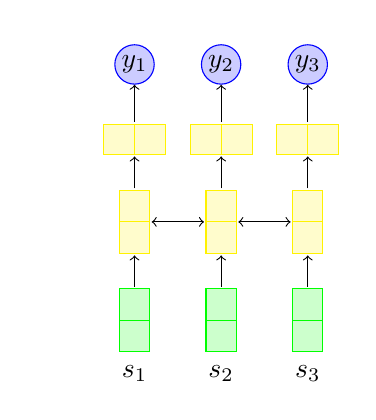
\begin{tikzpicture}[
  hid/.style 2 args={
    rectangle split,
    draw=#2,
    rectangle split parts=#1,
    fill=#2!20,
    outer sep=.25mm},
  mlp/.style 2 args={
    rectangle split,
    rectangle split horizontal,
    draw=#2,
    rectangle split parts=#1,
    fill=#2!20,
    outer sep=.25mm}
]

 % Comment out this line to remove border.
 \draw[draw=white] (-.25, 4.21) rectangle (3.8, -.4);

 \foreach \step in {1,...,3} {
   \node (i\step) at (1.1*\step, -.18) {$s_\step$};
   \node[hid={2}{green}] (e\step) at (1.1*\step, .5) {};    
 }
  
 \foreach \step in {1,...,3} {
   \node[hid={2}{yellow}] (h\step) at (1.1 *\step, 1.75) {};    
   \draw[->] (e\step.north) -> (h\step.south);
   
   \node[mlp={2}{yellow}] (g\step) at (1.1 *\step, 2.8) {};    
   \node[circle, draw=blue, fill=blue!20,minimum size=5mm] (y\step) 
       at (1.1 *\step, 3.75) {};
   \node at (1.1 *\step, 3.75) {$y_\step$};    
   \draw[->] (g\step.north) -> (y\step.south);
   \draw[->] (h\step.north) -> (g\step.south);
 }

 \foreach \last/\next in {1/2, 2/3} {
   \draw[<->] (h\last.east) -> (h\next.west);
 }


\end{tikzpicture}
\end{document}
